\documentclass{article}

\usepackage[utf8]{inputenc}
\usepackage[spanish]{babel}
\usepackage{csquotes}

\usepackage{graphicx}
\graphicspath{ {./img/} }
% \usepackage{ragged2e}

\usepackage[backend=biber,style=numeric]{biblatex}
\addbibresource{apt-bibliography.bib}
\hfuzz=14.999pt
\usepackage{hyperref}

\title{Impacto De APTs Sobre El Mundo Moderno}
\author{Giovanni Dueck\\\UrlFont{giodueck@gmail.com}\\\\{\bf Universidad Católica Nuestra Señora de Asunción}}
\date{Octubre, 2023}

\begin{document}

\maketitle

% Abstract
\begin{abstract}

Las amenazas cibernéticas que enfrenta el mundo de la informática hoy en día tienen una trayectoria de unos 30 años. Las amenazas relacionadas a gobiernos más antiguas datan a los años 90, y sus acciones influenciaron profundamente la forma en que funcionan las redes y computadoras hoy en día.

Esta investigación busca recopilar algunos de los grupos y eventos más significativos en el mundo de las Amenazas Persistentes Avanzadas, abreviadas {\it APT}, y cuales fueron los efectos que tuvieron sobre la tecnología moderna, el espionaje y el dominio de la guerra cibernética.

\end{abstract}

% Definiciones y glosario
\section{Definiciones}
\subsection{APT}
Una Amenaza Persistente Avanzada, o APT ({\it Advanced Persistent Threat} en inglés) es un actor sigiloso, típicamente un grupo perteneciente a o apoyado por un gobierno, que gana acceso no autorizado a una red de computadoras y permanece sin detectarse por un tiempo extendido. No se limitan a grupos apoyados por estados. \autocite{cybereason-apt} 

Una entidad se clasifica como APT si es:
\begin{itemize}
    \item {\bf Avanzada (Advanced)}: Los operadores detras del grupo poseen un espectro completo de herramientas de recolección de inteligencia. Incluyen herramientas propias y open-source, pero pueden también incluir a la organización de inteligencia del estado.
    \item {\bf Persistente (Persistent)}: Los operadores poseen objetivos a largo plazo, y no buscan información oportunísticamente por motivos de ganancia financiera u otros. Este tipo de objetivo sugiere que el atacante es guiado por una entidad externa. Los objetivos del atacante necesitan de un acceso permanente al objetivo, y al ser expulsados típicamente reintentan ganar acceso, y lo logran.
    \item {\bf Amenaza (Threat)}: Los atacantes son una amenaza porque tienen tanto capacidad como intención. Son manejados por acciones humanas y no simplemente por código automatizado. Son operadores capacitados, organizados y bien financiados. \autocite{itgov-apt}
\end{itemize}

\subsection{Arma Cibernética}
Comúnmente se refiere a malware empleado por parte de agencias militares, paramilitares o de inteligencia en un ataque cibernético. Esto incluye, entre otros, virus, trotanos, spyware y gusanos.

A diferencia de malware desarrollado para el crimen cibernético, como adware o ransomware, las armas cibernéticas típicamente son creadas por un APT o actor apoyado por un gobierno y pueden ser altamente selectivas en su objetivo. \autocite{stevens-cyberweapons}

\subsection{Ciberdelito}
Delito cibernético, o ciberdelito, es todo crimen o delito que involucra una computadora o redes de computadoras. Existen varias clases de crimen cibernético, desde fraude y lavado de dinero hasta crímenes financieros, estafas, extorsión, tráfico de drogas y materiales de abuso sexual de niños.

En la mayoría de los casos, el delito se comete con el fin de lucrar. Por lo tanto, en muchos casos, operaciones ejecutadas por APTs son especiales en el mundo del ciberdelito y son más similares al espionaje.

Se hará esta distinción en el resto del documento: una acción es claramente un ciberdelito si busca lucrar o ataca a la sociedad civil sin objetivos militares, de lo contrario típicamente se puede hablar de una guerra o arma cibernética. Aun así, veremos más adelante que esta distinción no siempre se puede hacer claramente. \autocite{cybercrime-britannica}

\subsection{Malware}
Malware ("malicious software", o software malicioso) es cualquier software diseñado para causar disrupción en una computadora, servidor, cliente o red, filtrar información privada, ganar acceso no autorizado, privar de acceso a información, o de otra forma irrumpe en la seguridad o privacidad informática de un usuario. \autocite{tahir-malware}

\subsection{Zero-day}
Un Zero-day (también escrito "0day") es una vulnerabilidad en un sistema informático desconocida por el proveedor y el público general. El nombre se refiere al tiempo que un proveedor conoce la vulnerabilidad.

Zero-days pueden ser explotados mientras no son conocidos por cualquier grupo para cualquier objetivo, incluyendo la infiltración de malware, spyware, o acceso indebido a información. Son mitigados mediante un parche por parte del proveedor, y una vez descubiertos empieza una carrera por el proveedor para lanzarlo. \autocite{symantec-zeroday}


% Breve listado
\section{Algunos APTs conocidos}
\subsection{China}
\subsubsection{APT1: Comment Crew}
APT1 es un grupo vinculado al Ejército Popular de Liberación (PLA por sus siglas en inglés) de China. Es uno de los principales y más conocidos APTs chinos, y ha realizado campañas de ciberespionaje, robo de secretos y robo de propiedad intelectual principalmente en los Estados Unidos.

El nombre coloquial de {\it Comment Crew} se debe a la tendencia a vulnerar sistemas de comentarios en sitios web legítimos. \autocite{bbc-comment-crew}

\subsubsection{APT10: Red Apollo}
APT10 se vincula comúnmente al Ministerio de Seguridad del Estado de China, y es más conocido por la operación Cloud Hopper, una campaña extensa de ataque y robo de información en múltiples países de todos los continentes que tenía como objetivo a proveedores de servicios gerenciados (Managed Service Providers, MSP). \autocite{trendmicro-cloud-hopper}

\subsubsection{APT41: Double Dragon}
APT41 es único entre los APTs chinos en que su operación es dual, operan tanto en campañas apoyadas por el gobierno como en campañas de cibercrimen, es decir para lucro del grupo, de donde provee el nombre {\it Double Dragon}.

Fueron nombrados por el Departamento de Justicia de los EE.UU. por haber comprometido a más de 100 empresas. \autocite{zdnet-apt41}

\subsection{Corea del Norte}
\subsubsection{APT38: Lazarus Group}
Lazarus Group es un grupo norcoreano designado tanto como APT como grupo criminal. Algunos investigadores reportan todos los casos de ataques provinientes de Corea del Norte bajo el nombre Lazarus Group, sin importar si provienen de algún subgrupo, como APT37 o Kimsuky. \autocite{mitre-lazarus}

Sus ataques más infames incluyen el ataque destructivo a Sony, robo al Banco de Bangladesh y el ransomware WannaCry. Sus operaciones incluyen activismo digital, espionaje y exfiltración de información, y crímenes financieros. \autocite{guardian-lazarus}

\subsection{Estados Unidos}
\subsubsection{Equation Group}
Equation Group es el grupo APT de la Agencia Nacional de Seguridad (NSA por sus siglas en inglés). Es actualmente considerado el APT más sofisticado, con operaciones que se adentran en el ciberespionaje, vigilancia masiva, y sabotaje por medio de armas cibernéticas capaces de causar daño en equipamiento industrial. \autocite{securelist-equation}

La NSA fue objetivo de mucha crítica el ser descubierto su rol en la creación de Stuxnet, considerada por muchos la primera arma cibernética, por ende iniciando la era de las guerras cibernéticas, y por las tácticas y herramientas que tienen a su disposición, que fueron descubiertas por varios leaks. \autocite{washingtonpost-stuxnet}

\subsection{Iran}
\subsubsection{APT33: Elfin Team}
APT33 es un grupo formado a más tardar en 2013, demostrando una gran capacidad de crecimiento en el área de seguridad por parte del gobierno iraní. Los objetivos de este grupo son principalmente los EE.UU. y Arabia Saudita, con el ataque más conocido deshabilitando las operaciones de la mayor empresa de petroquímicos de la zona, Saudi Aramco. \autocite{mandiant-apt33}

\subsection{Israel}
\subsubsection{Unit 8200}
Unit 8200 es una unidad de los Cuerpos de Inteligencia de Israel cuya misión es la captación y descifrado de códigos. Frecuentemente son asociados con Stuxnet, ciberarma en cuya creación Israel colaboró con la NSA de los EE.UU. \autocite{washingtonpost-stuxnet}

La unidad se compone principalmente de jóvenes de entre 18 y 21 años de edad, debido a, servicio militar obligatorio de no más de dos años. Esto significa que los reclutas elegidos deben tener la capacidad de aprender rápidamente y ser de utilidad a la unidad en el tiempo restante. Muchos ex miembros van al mundo empresario, con varios de estos fundando grandes empresas como Wix y NSO Group, y muchos otros trabajando en las mayores empresas tecnológicas del mundo. \autocite{globes-unit-8200} \autocite{forbes-unit-8200}

\subsection{Rusia}
\subsubsection{APT28: Fancy Bear y APT29: Cozy Bear}
APT28 y APT29 son dos grupos primariamente de ciberespionaje. Sus operaciones más conocidas son las interferencias en las elecciones de los EE.UU. en 2016, aunque también atacaron a varios países europeos y a la Agencia Mundial del Antidopaje. \autocite{sslstore-apt28-apt29}

\subsubsection{Sandworm}
Este grupo realizó varias operaciones contra el ejército y el pueblo de Ucrania, con ataques a la red eléctrica y un wiper que arrazó con una gran mayoría de los sistemas informáticos del país, considerado el ataque cibernético más destructivo de la historia. También emplearon un malware destructivo para atacar a los juegos olímpicos de invierno de 2018, haciendo todo lo posible para evitar ser descubiertos. \autocite{wired-notpetya} \autocite{wired-olympic-destroyer}


% Eventos
\section{Eventos y operaciones}

\subsection{Moonlight Maze (1996)}
En 1996, uno de los primeros ataques cibernéticos masivos había comenzado. Un grupo de hackers exfiltró una cantidad monumental de documentos, que si fuesen impresos y apilados superarían los 160 metros de altura. \autocite{securelist-moonlight-maze}

Un equipo de investigación fue formado en 1999, y la investigación recibió el nombre de "Moonlight Maze". Se recolectó mucha evidencia, pero la mayoría fue clasificada o dejada fuera de las manos del público, pero una investigación reciente por parte de un equipo en Kaspersky reveló tácticas y herramientas que muestran conexiones con un grupo moderno: Turla.

Turla es un APT ruso cuya operación de ciberespionaje en 2014 fue descubierta por Kaspersky e investigada extensamente. Los ataques se aprovecharon de dos zero-days, además de varias vulnerabilidades ya resueltas, y el malware infectó a computadoras en más de 45 países mediante tácticas de ingeniería social y spear-phishing. \autocite{securelist-turla}

Vincular a un grupo sofisticado como Turla con un ataque tan histórico como lo es Moonlight Maze, revela que el grupo es realmente uno de los más antiguos y experimentados APTs existentes. El único grupo de edad similar es Equation Group, el APT vinculado con la NSA. Este último ya estuvo activo en 2001, y tal vez hasta en 1996. \autocite{securelist-equation}

Ataques de esta magnitud muestran que los APTs bien financiados y capaces no son un fenómeno nuevo, existen desde los comienzos del internet. Moonlight Maze estableció el estándar del arsenal de herramientas del atacante moderno. 

\subsection{Titan Rain (2000s)}
En 2005 se revelaron una serie de ataques a varias instituciones de los gobiernos de los Estados Unidos y del Reino Unido, los cuales se sospechan que empezaron en 2003. El Reino Unido reportó que la campaña continuaba activa hasta 2007. \autocite{cfr-titan-rain}

Shawn Carpenter, un analista de seguridad informática en Sandia National Laboratories, laboratorio en el cual parte del arsenal nuclear americano es diseñado, descubre en 2003 una intrusión. En Lockheed Martin, una empresa de aeronáutica americana, el mismo actor logra infiltrarse y acceder a documentos sensibles relacionados a varios proyectos militares de la empresa.

Carpenter inicia una campaña propia para rastrear a los intrusos en su tiempo libre, actuando de informante para el gobierno. Increíblemente, Carpenter logra ubicar a los intrusores en la China. Según él, este grupo "nunca presionó una tecla equivocada." Sin duda, se trataba de un actor militar.\autocite{time-titan-rain} \autocite{homelandsecurity-titan-rain}

Como la operación de Carpenter no tenía una autorización, la FBI compartió los datos de su intervención en la investigación con Sandia, de la cual fue despedido. En respuesta, Carpenter lanza una demanda y gana US\$ 4,3 millones, con el juez recalcando que este fue un acto patriótico por el cual no debió haber sido castigado.

El incidente recalcó la importancia de una actitud de la no ignorancia con respecto a la seguridad informática, y solidificó la noción de que el espionaje moderno cambió del dominio físico al digital. \autocite{computerworld-titan-rain}

\subsection{Operation Aurora (2010)}
En enero de 2010, Google anunció que habían descubierto una intrusión en diciembre de 2009. Proviniendo de China, los ataques afectaron a 34 empresas de diversos sectores, desde internet a finanzas a fabricantes de químicos. 

Los datos robados fueron principalmente propiedad intelectual, llevando a la especulación que el gobierno chino buscaba robar productos y tecnología americanos. Pero su objetivo en Google era principalmente el acceso a varias cuentas de Gmail pertenecientes a activistas de derechos humanos chinos. Además, Google descubrió que varias cuentas de activistas de alrededor del mundo sufrieron accesos no autorizados rutinarios en sus cuentas de Gmail. \autocite{google-aurora}

De acuerdo a McAfee, los atacantes tuvieron acceso al código fuente de varias empresas tecnológicas y del sector de defensa. En el centro del escándalo estaban los sistemas de gestión de configuración de software (SCM por sus siglas en inglés), que no tenían defensas. Esto significa que las vulnerabilidades en los productos de estas empresas pueden ser encontradas más facilmente al tener acceso al código fuente. \autocite{wired-aurora}

\subsection{Stuxnet (2010)}
Stuxnet es el malware más sofisticado jamás encontrado. Según varios reportes, es la obra de las agencias de inteligencia de los Estados Unidos e Israel, y es generalmente considerada la primera arma cibernética y el incidente que inició la era de la guerra cibernética.

Inicialmente, expertos encontraron versiones que datan a junio de 2009, y más tarde se encontrarían versiones en uso desde 2007. Sin embargo, es la versión final descubierta en 2010 que hacía uso de varios {\it exploits} \footnote{Del inglés. Un {\it exploit} es un fragmento de software utilizado en la explotación de una vulnerabilidad de software} críticos de Microsoft Windows y poseía capacidades impensables para la época. Con un total de cuatro zero-days, Stuxnet es de complejidad incomparable. Donde un malware común normalmente emplea tácticas de ingeniería social y no más de un zero-day, aquí se emplean cuatro en un solo ataque. \autocite{symantec-stuxnet} \autocite{reuters-stuxnet}

\subsubsection{Historia}
La misión de Stuxnet era una de sabotaje como alternativa a un conflicto tradicional. Los EE.UU. habían descubierto que Irán, por medio de un físico llamado A.Q. Khan en Pakistan, lanzó un programa de enriquecimiento nuclear entre 1998 y 1999 y comenzó a comprar diseños para una fábrica de centrífugas. La CIA y la inteligencia británica habían infiltrado la cadena de suministro de A.Q. Khan y lograron interceptar un envío de centrifugas a Libia. En 2004, la Agencia Internacional de Energía Atómica de las Naciones Unidas investigó al programa libio y la CIA adquirió los materiales del programa.

Las centrífugas se estudiaron extensivamente, lo que permitió crear un virus sigiloso que es capaz destruir equipamiento industrial físico, por primera vez en la historia. Con estos hallazgos, las administraciones del presidente Bush y más tarde la del presidente Obama aprobaron el programa, que fue nombrado Operación {\it Olympic Games} (Juegos Olímpicos).

La versión inicial, sin embargo, tenía una falta: no lograba alcanzar a todas las computadoras necesarias, las que controlaban al sistema de control industrial. Por este motivo se agregaron exploits agresivos que permitieron al virus (1) esparcirse por la red local de una máquina infectada, (2) obtener privilegios elevados y (3) esconder la presencia y acciones del sistema operativo. Esta clase de malware es llamada un {\it worm} (gusano), un programa que es capaz de replicarse de forma autónoma para moverse a huéspedes nuevos, y las herramientas que permiten esconderse del sistema operativo y obtener privilegios elevados son llamadas {\it rootkit}.

El ataque inició con una infiltración física del malware a la planta nuclear Natanz, que se encuentra en una zona remota y desconectada de internet. Una vez que Stuxnet logra infectar a la primera máquina, infecta rápidamente a toda computadora con Windows en la red en busca de instalaciones de software Siemens para el control de las centrífugas. Una vez encontradas estas computadoras críticas, monitorea el comportamiento normal de los sistemas de control antes de interferir en su operación. Un diagrama delinieando este proceso se muestra en la figura \ref{fig:stuxnet}.

Stuxnet era capaz de alterar las frecuencias a las que operaban las centrífugas; al mismo tiempo reportaba frecuencias normales al sistema de monitoreo. De esta forma, las centrífugas se desgastan y hasta autodestruyen mucho más rápidamente. Se estiman que alrededor de 1.000 centrífugas fueron dañadas durante la operación, y el gas de uranio que contenían, desperdiciado. \autocite{zetter-stuxnet} \autocite{washingtonpost-stuxnet}

El virus finalmente fue descubierto por analistas de VirusBlokAda, un proveedor de antivirus, al escapar de la planta por medio de una computadora transportada fuera del predio. Un reporte por Symantec luego afirmó que computadoras alrededor del mundo habian sido infectadas, con la gran mayoría de ellas en Irán. Se reportaron también que varios de los exploits utilizados ya se habían encontrado anteriormente por otras operaciones del APT Equation Group, por lo cual el ataque les fue atribuído. \autocite{infoworld-stuxnet} 

Stuxnet inició debates sobre la guerra en el plano de la información. Fue la primera vez que un virus mostró la capacidad de subvertir sistemas de control industrial de manera tan sofisticada. Hasta este punto, la guerra cibernética no se había definido. El hecho de ser un ataque cibernético otorga cierta negación plausible (que no es posible con un ataque con misiles o bombas), y tampoco es claro si un ataque cibernético constituye un acto de guerra. \autocite{washingtonpost-stuxnet-2} \autocite{darknetdiaries-stuxnet}

\begin{figure}[t]
    \centering
    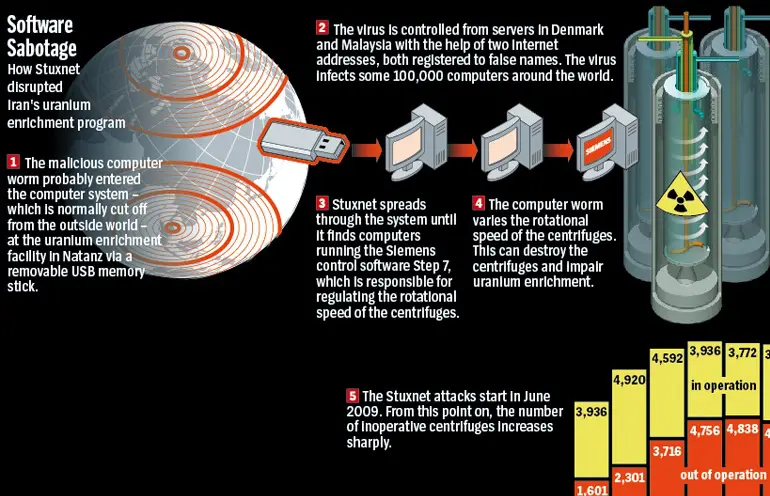
\includegraphics[width=1.0\textwidth]{Stuxnet_jpg.png}
    \caption{funcionamiento de Stuxnet \autocite{extremetech-stuxnet}}
    \label{fig:stuxnet}
\end{figure}

\subsection{Sony (2014)}
En respuesta a la producción de la película satírica {\it The Interview}, Sony Pictures fue hackeada en 2014 por operativos de Corea del Norte. El ataque consistió en el robo de información, entre otros sobre obras en producción y datos de empleados, y la implantación de un virus {\it wiper} \footnote{Del inglés. {\it Wipers} son una clase de malware cuyo objetivo es la destrucción de datos y/o sistemas informáticos}.

Mientras que este ataque fue el que puso a Corea del Norte en el mapa, el grupo autodenominado {\it Guardians of Peace} (Guardianes de la Paz) mostró signos de actividad desde al menos 2009 y parece ser responsable de más de 45 familias de malware. El ataque a Sony demostró una capacidad que no pudo haber aparecido en solo un año.

Hoy en día el grupo es mejor conocido como Lazarus Group. Hasta este momento no parecía ser un grupo muy sofisticado, con métodos crudos y operaciones de magnitud limitada, pero no lo necesitaba ser. Con las herramientas que poseían, ya demostraban ser un grupo peligroso y capaz de alcanzar sus objetivos. \autocite{wired-sony}

El mismo grupo continuó su trayectoria de ciberespionaje y extorsióna a través de las numerosas campañas que le siguen a esta primera.

\subsection{Banco de Bangladesh (2016)}
En 2016, Lazarus Group se infiltró en el Banco de Bangladesh y realizó transferencias SWIFT de casi US\$ 1.000 millones a varias cuentas bancarias pertenecientes al grupo en diversos bancos, algunos de ellos en las Filipinas. Sin embargo, un error de tipografía en las intrucciones de transferencia detectado por un empleado bancario realzó sospechas, por lo que la mayoría de las transferencias fueron bloqueadas. El monto robado terminó siendo de alrededor de US\$ 81 millones.

El 4 de febrero, los hackers lograron enviar más de tres docenas de transferencias fraudulentas usando credenciales del sistema SWIFT del Banco de Bangladesh. US\$ 81 millones fueron enviados exitosamente a varias cuentas bancarias en las Filipinas, mientras que la mayor parte, unos US\$ 850 millones, fue bloqueada al encontrar un error en la instrucción de transferencia.

El Banco de Bangladesh pudo descubrir el robo gracias a un error de una impresora, la cual estaba configurada para imprimir un registro constante de cada transferencia SWIFT realizada pero había fallado durante el ataque. Al finalmente reiniciar la impresora, se dieron cuenta de las transferencias realizadas. El Banco de la Reserva Federal de Nueva York había intentado contactar con el Banco de Bangladesh, pero nadie respondió gracias al fin de semana en el país. Cuando intentan contactar a SWIFT y a Nueva York para responder a los mensajes, nadie respondió gracias al fin de semana en los EE.UU. Cuando al fin logran establecer las comunicaciones el lunes siguiente, descubren que varias de las transferencias han sido aprobadas: un total de US\$ 101 millones. Intentos de contactar con el banco RCBC de las Filipinas también se atrasaron por un día feriado, el año nuevo chino. \autocite{wired-bangladesh} \autocite{nypost-bangladesh}

US\$ 20 millones fueron recuperados más tarde, pero Lazarus continuó sus planes con los demás US\$ 81 millones. Por medio de unos apostadores chinos, el dinero se lava y desaparece. \autocite{bloomberg-bangladesh}

Lazarus Group ahora ya no es solo un grupo de espionaje, sabotaje y extorsión, sino también un grupo criminal. Con la cantidad limitada de comercio exterior del país marginado, y con la serie de otros ataques similares menores, el dinero robado por parte del programa de hackers norcoreano debe componer una buena parte del producto interno bruto anual. Esto hace a Corea del Norte el único APT que realiza operaciones netamente cibercriminales y el único estado con el robo como significante contribuyente a la economía.

% \subsection{Interferencia de Elecciones (2016)}
% Todo only if got time

\subsection{The Shadow Brokers (2016)}
En agosto de 2016, un grupo nuevo anunció que había hackeado a la NSA. Específicamente, afirmaban haber hackeado a Equation Group y robado numerosas ciberarmas. Este grupo se llamaba {\it The Shadow Brokers} \footnote{en inglés, {\it shadow} significa sombra, y {\it broker} significa corredor o agente de bolsa y se refiere a un negociante.}.

Shadow Brokers realizaron muchas afirmaciones exageradas, incluso que las herramientas robadas eran mejores que Stuxnet, pero resultó ser cierto que estas herramientas debían proveer de Equation Group, específicamente la unidad entonces llamada TAO. \footnote{en inglés, {\it Tailored Access Operations}, operaciones de acceso a medida, es una unidad especializada en el desarrollo de tanto hardware como software de espionaje e infiltración cibernética. El nombre actual de la unidad es {\it Computer Network Operations}.} \autocite{sophos-shadow-brokers}

Inicialmente solo disponibilizaron unas pocas muestras, con la intención de subastar el resto al mejor postor, o al público general si el total de las ofertas llegase a BTC 1.000.000 (alrededor de US\$ 600 millones en ese tiempo). Pero como no lograron recaudar un monto significante, el grupo decidió publicar las herramientas descubiertas al público general.

Hacer de acceso público armas cibernéticas sofisticadas, algunas incluso datando a los años 90 y las más recientes a 2013, significó un riesgo importante al mundo entero. Ahora no solo APTs podían acceder a armas cibernéticas sofisticadas, sino grupos de criminales comunes.

Además, Shadow Brokers demostraron también que posían información operacional. Jake Williams, fundador de Rendition Security, publicó bastante sobre el grupo. En respuesta, un mensaje dirigido a Williams lo expuso como ex miembro de Equation Group, lo cual era información clasificada, y este lo confirma. \autocite{nytimes-shadow-brokers} \autocite{darknetdiaries-shadow-brokers}

La NSA tiene una mala racha de ser expuesta por sus operaciones. Primero, Stuxnet escapa de su objetivo para luego infectar al mundo y exponer las capacidades de creación de ciberarmas de Equation Group. Luego, en 2013 Edward Snowden, ex contratista de la NSA, filtra miles de documentos revelando las capacidades de ciberespionaje y programas vigilancia masiva de la agencia. Ahora, hackers logran acceder a y distribuir herramientas altamente peligrosas, las cuales la NSA ha estado acumulando desde los años 90 sin contactar a los proveedores de los productos afectados.

Esta última tendencia, la de acumular exploits para su uso en ciberarmas, se vio especialmente criticada en los años posteriores a este incidente por autores y periodistas. \autocite{schneier-shadow-brokers}. El exploit más significante del conjunto, nombrado \textsc{EternalBlue}, causó graves daños al ser usado por Lazarus Group de Corea del Norte y Sandworm de Rusia en ataques masivos que lograron llevar a algunas de las empresas y agencias de gobierno más grandes del mundo a la era del lapiz y papel. Curiosamente, un parche para la vulnerabilidad fue lanzada poco tiempo antes de que el exploit sea revelado al público, llevando a especular que la NSA advirtió a Microsoft una vez que se enteraron de la brecha.

\subsection{WannaCry (2017)}
En mayo de 2017, el ciberataque más devastador hasta entonces empezó. Un ransomware llamado WannaCry, usando el exploit \textsc{EternalBlue}, se estaba propagando por las computadoras de organizaciones e individuos, encriptando archivos, y demandando un pago por la recuperación de la información.

\begin{figure}[t]
    \centering
    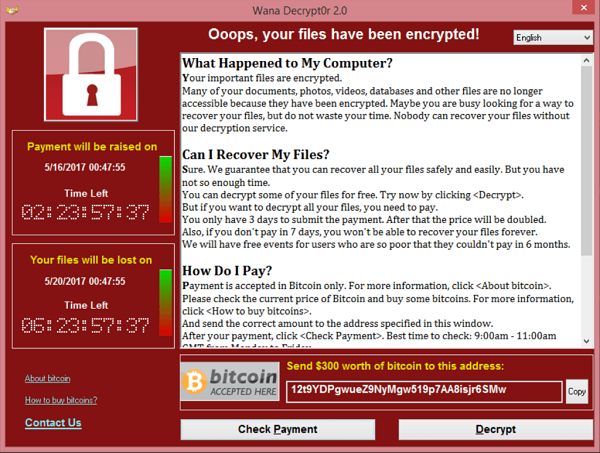
\includegraphics[width=0.8\textwidth]{Wana_Decrypt0r.png}
    \caption{pantalla de una computadora infectada con el ransomware WannaCry}
\end{figure}

\textsc{EternalBlue}, una de las ciberarmas de la NSA robadas por los Shadow Brokers, se aprovecha de una vulnerabilidad de ejecución remota de código en el protocolo de transferencia de archivos SMB en Windows. MS17-010, como la llamó Microsoft, es una vulnerabilidad tan severa que hasta productos viejos sin garantía de soporte recibieron un parche para mitigarla, y WannaCry demostró por primera vez esta severidad a gran escala. \autocite{mandiant-mannacry}

Dentro de pocos minutos, el virus es capaz de infectar una organización entera. Entre las afectadas está la NHS, el servicio nacional de la salud del Reino Unido. Este se vió obligado a desconectar a varios hospitales del internet, varios otros tuvieron que suspender sus actividades o continuarlas en papel y pizarras. 

El virus consiste de dos módulos: un gusano, que mediante \textsc{EternalBlue} se propaga a nuevas máquinas, descarga y ejecuta las herramientas para ejecutar el ataque sobre los archivos, y las herramientas de encripción, que causan un daño crítico a los archivos de una computadora. Finalmente, una pantalla de ransomware informa a la víctima de su destino y propone las instrucciones para la decodificación de sus archivos: un pago de US\$ 300 a US\$ 600 en Bitcoin.

Sin embargo, el virus posee un punto débil. Un {\it killswitch}, un interruptor de apagado, que consiste en una prueba de conexión a una URL de nombre aparentemente aleatorio. Cuando un analista independiente registra el nombre de dominio unas horas luego del inicio del ataque, encuentra que al lograr conectarse, el virus desactiva la herramienta de encripción y detiene el ataque. Múltiples versiones aparecieron luego de activarse el killswitch, tanto con un URL diferente como sin killswitch, pero ya no llegaron a causar el mismo impacto que la primera oleada. \autocite{darknetdiaries-wannacry}

El Departamento de Justicia de los Estados Unidos comunicó a la prensa en 2018 una acusación a un programador de Corea del Norte por su participación en Lazarus Group y los ataques a Sony, robo al Banco de Bangladesh y ataque WannaCry. \autocite{doj-lazarus}

\subsection{NotPetya (2017)}
Antes de la invasión a gran escala, Rusia invadió a Ucrania en 2014 y anexó al territorio de Crimea. Desde entonces, ha ocupado el territorio de Donbas y está causando sufrimiento para el país ex soviético, que en el pasado se había llamado el granero de la Unión Soviética.

Entre 2014 y 2022 ha regido un caos en el plano cibernético, el cual expertos clasifican como la primera guerra cibernética real. El grupo Sandworm, un APT operado por la unidad militar 74455 de la GRU, el servicio de inteligencia militar de Rusia, llevó a cabo varios ataques cibernéticos sobre la infraestructura militar y civil de Ucrania. Entre los primeros, están varios ataques destructivos a la red eléctrica del país en 2015 y 2016. \autocite{doj-sandworm}

\begin{figure}[t]
    \centering
    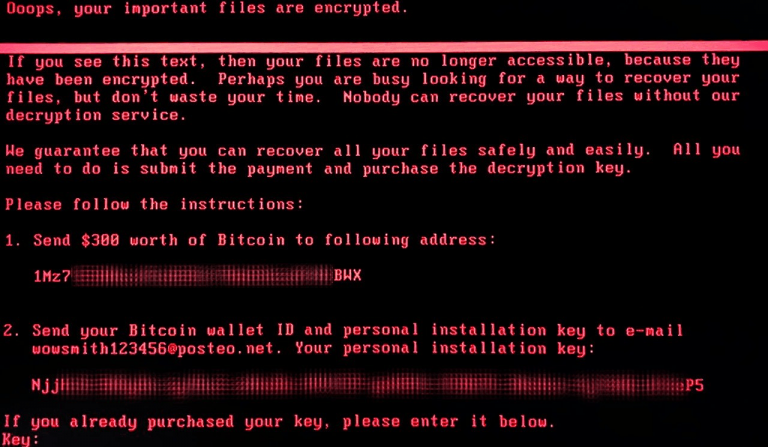
\includegraphics[width=1.0\textwidth]{notPetya.png}
    \caption{pantalla de una computadora infectada con el wiper NotPetya}
    \label{fig:notpetya}
\end{figure}

En 2017, Sandworm lanza el virus más tarde denominado "NotPetya" \footnote{un ransomware llamado Petya fue usado como la base de este ataque, pero las modificaciones eran sustanciales tanto en su rutina de encripción como en su forma de propagación. Por esta razón, Kaspersky lo llamó ExPetr, o NotPetya. \autocite{kaspersky-notpetya}} por medio de una actualización maliciosa al programa M.E.Doc, un servicio al cual se habían infiltrado unos meses antes. M.E.Doc es un software para el manejo de impuestos en Ucrania, por lo que una infección a este programa resultaría en una infección a la nación entera. Para infectar a las demás computadoras, se empleó una versión modificada de \textsc{EternalBlue}, el mismo exploit usado en WannaCry, y el exploit \textsc{EternalRomance}, también del paquete filtrado por Shadow Brokers.

En realidad, NotPetya no era realmente un ransomware, ya que los autores no proveían los datos necesarios para generar una clave de decodificación. Esto significa que en realidad era un {\it wiper}, con el objetivo de destruir datos y sistemas informáticos a escala masiva, tanto en empresas como instituciones públicas.

Residentes de Ucrania perdieron acceso al pago electrónico del transporte público y la mayoría de los ATMs, supermercados perdieron la habilidad de vender sus productos ya que las cajas se encontraban mostrando una pantalla como en la figura \ref{fig:notpetya}. Todo servicio ucraniano conectado directa o indirectamente a internet se vió afectado.

Pero un worm no conoce límites geográficos. Aunque la mayor parte de las infecciones se dieron en Ucrania, Rusia también se vió muy afectada ya que tenía muchas conexiones con Ucrania. Empresas multinacionales con sedes en Ucrania también fueron atacadas. \autocite{securelist-notpetya}

Uno de los casos más destructivos es el de Maersk, la empresa de transporte marítimo. Esta perdió la gran mayoría de sus sistemas informáticos, lo que causó filas de decenas de miles de camiones con pedidos que no podían completar, en algunos casos de productos perecederos. Barcos llenos de contenedores llegaban a puertos, pero nadie sabía qué carga tenían los contenedores. El incidente casi destruyó a la empresa, y causó la reconstrucción total de su infraestructura de TIC. \autocite{darknetdiaries-notpetya}

Andy Greenberg, un experto en el grupo Sandworm, llamó al ataque de NotPetya el más destructivo de la historia. Ataques de esta escala brindan un ejemplo de lo que es la guerra cibernética, y de lo que son capaces los grupos APT cuando tienen acceso a armas cibernéticas de grado militar como lo fue \textsc{EternalBlue}. \autocite{wired-notpetya} \autocite{greenberg-sandworm} 

% \subsection{Olympic Destroyer (2018)}
% TODO only if got time olympic destroyer

\subsection{SolarWinds (2020)}
En diciembre de 2020, Fireeye descubrió una intrusión en sus sistemas que compartió con el mundo. El ministerio de defensa estadounidense inició una investigación relacionada a una brecha similar en sus sistemas, asi también empresas como Microsoft y Mandiant. \autocite{wired-solarwinds} \autocite{npr-solarwinds}

La investigación rápidamente concluyó que el actor mostraba señales de ser un grupo ruso, cuyo objetivo era principalmente el ciberespionaje antes que la destrucción. En 2022, Mandiant reveló al actor, llamado {\it Dark Halo} y {\it UNC2452}, como APT29, también conocido como Cozy Bear.

Entre marzo y mayo, los atacantes logran infiltrarse en los sistemas de la empresa SolarWinds, la cual provee Orion, un producto de monitoreo de redes. Este producto es usado en muchas empresas importantes de diversos sectores, como Fireeye y Microsoft, y en muchas organizaciones gubernamentales.

El ataque consiste de un troyano de acceso remoto, o RAT. Una actualización se publica con código malicioso, llamado \textsc{Sunburst}, que permite a los atacantes acceder a cualquier sistema de forma sigilosa. Para evitar que se descubra la manipulación del código, los atacantes incluyeron fragmentos de software en el proceso de construcción de Orion. Esto permitió inyectar el código malicioso sin modificar el código legible por humanos, antes de generar la firma digital que previene la modificación posterior de la herramienta y que asegura que el producto no fue manipulado.

Un ataque de este tipo se denomina un ataque de cadena de suministro, y con los miles de clientes se lograría atacar a muchos objetivos de forma sencilla. Protegerse de este tipo de actores implica, por lo tanto, no solo verificar los sistemas y productos propios de una organización, sino también la verificación de toda herramienta proveída por terceros. Se estima que unos 18.000 clientes fueron infectados, de los cuales alrededor de mil fueron atacados.

Entre las víctimas más importantes se encuentra Fireeye, una empresa de ciberseguridad, que estimó que muchas herramientas de testeo de penetración, es decir herramientas de hackeo, fueron robadas. 

Con ocho meses entre la infección inicial y la detección, el ataque reveló el aumento drástico en las capacidades de APT29. Revela también un nuevo nivel de sofisticación en la seguridad operacional (OPSEC) de grupos adversarios, un alto grado de persistencia y un abordaje cada vez más agresivo a la recolección de información. El presidente de Fireeye afirmó que el ataque a SolarWinds fue uno de los más sofisticados visto en la historia de la empresa. \autocite{fireeye-solarwinds} \autocite{mandiant-solarwinds}

El presidente de los EE.UU. Joe Biden respondió con medidas y sanciones agresivas de una manera no vista frecuentemente. El ataque fue comparado con Moonlight Maze por varios analistas de seguridad y como una declaración implícita de guerra por otros, reforzando la retórica de disuación por medio de medidas contra actores cibernéticos hostiles. Este tipo de ataques surgen como la mejor, y tal vez la única, alternativa a un ataque convencional, ya que los EE.UU. poseen las fuerzas militares más poderosas del mundo. \autocite{cnbc-solarwinds}

\subsection{Axie Infinity (2022)}
En marzo del 2022, el creador del juego basado en criptomonedas y NFT {\it Axie Infinity} anunció que había descubierto una brecha. Esta resultó en el robo de unos US\$ 620 millones, el robo de criptomonedas más grande de la historia. En abril, autoridades estadounidenses anunciaron que vincularon una de las direcciones de billetera a Lazarus Group. \autocite{washingtonpost-axie}

La fundación del juego es la blockchain llamada Ronin Network, creada con juegos en mente. A diferencia de una cadena como la de Bitcoin, Ronin se diseñó con la intención de soportar una gran cantidad de transacciones por segundo. Para alcanzar este objetivo, un método de validación de bloques de prueba de trabajo (comúnmente llamada minería) sería poco ideal por la gran cantidad de trabajo desperdiciado para las frecuentes transacciones que implica el diseño de un videojuego. En su lugar, Ronin utilizaba un sistema llamado Prueba de Autoridad, en donde nodos llamados {\it validadores} votan para aprobar bloques nuevos de transacciones. \autocite{ronin-intro}

Los hackers que penetraron a Sky Mavis, la empresa desarrolladora del juego, notaron que cuatro del total de nueve claves validadoras se encontraban en manos de la empresa. Como cuatro de nueve no superan la mitad de los validadores, era necesaria una clave más para forjar transacciones ilícitas; es para estos casos que existen multiples nodos validadores. 

En 2021, Sky Mavis fue otorgada acceso al validador de la organización descentralizada autónoma (DAO por sus siglas en inglés, {\it Decentralized Autonomous Organization}) de Axie Infinity para ayudar al DAO a distribuir transacciones libres de tarifas por una inmensa carga de usuarios. Como el permiso de operar esta clave no fue denegado al volver a la normalidad, los hackers lograron acceder a la clave, en efecto otorgándose la autoridad de votar por transacciones ilegales de retiros de fondos. \autocite{ronin-axie}

Una diferencia clave entre las finanzas tradicionales y las descentralizadas es que las transacciones en blockchain son irreversibles. En el robo al Banco de Bangladesh, la gran mayoría de las transacciones ilegales del sistema SWIFT fueron bloqueadas. Esto es imposible con blockchain por diseño; la cadena no puede ser modificada y no miente. Transacciones aprobadas en cryptomonedas no son reversibles, lo que hace a este mundo un objetivo interesante tanto para estafas como robos. \autocite{chainsec-axie}

Investigadores notaron que Lazarus robó alrededor de US\$ 400 millones en 2021, haciendo a este incidente particularmente lucrativo para el gobierno de Corea del Norte. El grupo ha mostrado la capacidad de penetrar cualquier industria, ya sea de entretenimiento en el caso de Sony, bancos centrales como el de Bangladesh, o monedas descentralizadas como en el caso de Ronin Network. El ataque evidenció que ninguna empresa y ningún sistema es inmune a las amenazas cibernéticas. \autocite{washingtonpost-axie}

\section{Efectos y consecuencias}
En general, las acciones tanto de APTs como de cibercriminales han causado un enfoque mundial aumentado en ciberseguridad. Gobernantes expresan la necesidad de declarar ciertos sectores como fuera de los límites de ciberataques, varias alianzas y gobiernos han definido sanciones a ciberataques o se reservan el derecho de responder con ataques tradicionales, y las Naciones Unidas reconocen la necesidad de crear un conjunto de reglas de combate análogas al Convenio de Ginebra. \autocite{cfr-regulations}

Las empresas han empezado a reconocer que deben invertir en seguridad, aun si no son objetivos militares, y las personas se muestran más atentas a invasiones de privacidad.

Estas consecuencias, tanto directas como indirectas, se evidencian en casi todos los sectores de la industria, el gobierno y la sociedad civil.

\subsection{Erosión de confianza}
Las acusaciones y contra-acusaciones de ataques cibernéticos entre países causa una erosión de confianza que puede aumentar tensiones y causar más conflicto.

Esta erosión no se limita a países con rivalidades, como los Estados Unidos con Rusia o China, sino que se da entre países aliados también. En respuesta a la revelación del programa de vigilancia de la NSA por parte de Edward Snowden en 2013, muchos ciudadanos de diferentes países, incluyendo los EE.UU., salieron a protestar. Varios países europeos criticaron fuertemente al programa. De entre ellos, Alemania con su historial de dictadura y control poblacional fue el crítico más fuerte. Se reveló que el teléfono de la canciller Angela Merkel estaba entre los objetivos de la NSA, lo que llevó a crítica, investigación, y acusación pública por parte del gobierno hacia los EE.UU. y sus instituciones en Europa. \autocite{wiki-reaction-snowden}

\subsection{Impacto económico}
Varios ataques tuvieron impactos enormes en la economía. El ataque NotPetya deshabilitó una buena parte de la infraestructura básica de Ucrania, incluyendo ATMs y sistemas de transporte público, y costó unos US\$ 2,3 mil millones a las mayores empresas afectadas por el virus. \autocite{wired-notpetya}

Ataques a bancos y redes de criptomonedas hackeadas tienen un efecto inmediato, con varios millones en transacciones bancarias fraudulentas y muchos miles de millones en criptomonedas robadas hasta la fecha. \autocite{wired-bangladesh} \autocite{chainsec-axie}

Impactos más sutiles se presentan al realizar entrenamientos y mejoras en sistemas informáticos. Empresas que investigan o se recuperan de un ataque gastan, en ocasiones, millones en su infraestructura. Otras empresas invierten grandes cantidades para evitar convertirse en víctimas en el futuro. \autocite{wiki-reaction-snowden}

En otros casos, países han roto acuerdos económicos. Un ejemplo es Ecuador, que en respuesta al programa de vigilancia de la NSA renunció a beneficios del comercio con los EE.UU. valorados en más de US\$ 20 millones anuales. \autocite{wiki-reaction-snowden}

\subsection{Impacto en privacidad}
Desde las revelaciones de Snowden, la cultura de la privacidad digital ha existido para brindar una forma de aprovechar los derechos humanos.

Algunos impactos fueron culturales: en Alemania se ha vuelto un hábito tapar cámaras web en computadoras. Otras recomendaciones, como la de no confiar en correo electrónico, cookies, o políticas de privacidad vagas, todavía no son bien entendidas por el público general o están en proceso de convertirse en conocimiento común.

Aun así, la falta de consideración de la privacidad es la principal vulnerabilidad que explotan muchos ataques de spearphishing, una de las técnicas utilizadas por ejemplo en el ataque a Axie Infinity, para forjar mensajes convincentes para engañar a la víctima. Ataques de phishing en general son mucho más efectivos una vez que se aprovechan de la falta de privacidad del mundo actual. \autocite{ronin-axie}

\subsection{Vulnerabilidades de la cadena de suministro}
Los ataques recientes a SolarWinds y su posición como proveedor de software para muchas empresas y organizaciones importantes para la seguridad nacional estadounidense causó un debate sobre la confianza que se otorga a los proveedores de software.

Es evidente que la verificación detenida de todo software proveniente de terceros, además de los propios sistemas y productos informáticos, es imposible. El estándar de seguridad para estas empresas y sus productos debe ser más alto. Se estima que de alrededor de 100 instituciones víctimas del ataque fueron infiltradas y aprovechadas para el espionaje, y que además muchas de estos accesos pudieron a su vez haberse convertido en ataques a sus respectivas cadenas de suministro. \autocite{wired-solarwinds} \autocite{npr-solarwinds}

\subsection{Proliferación de armas cibernéticas}
La revelación de la existencia de Stuxnet y su posterior análisis reveló al mundo que ataques cibernéticos son capaces de causar daños a equipos físicos y hasta personas. Aunque Stuxnet no causó muertes según lo reportado, otros virus con sistemas de control industrial podrían afectar el manejo de gases peligrosos, tanques que manejan presiones enormes, o todo tipo de equipamiento potencialmente mortal.

Los países con las capacidades para desarrollar este tipo de malware ya lo están haciendo por más de una década, y otros países rápidamente desarrollaron estas capacidades en respuesta. Irán desarrolló malware en respuesta a Stuxnet, el wiper Shamoon, en cortísimo tiempo, y Corea del Norte empezó a adentrarse en el campo alrededor de ese tiempo también. \autocite{darknetdiaries-stuxnet} \autocite{infosecurity-cyberwar}

Una gran desventaja de las armas cibernéticas es que no tienen el mismo poder de disuasión de las armas tradicionales. Las bombas nucleares solo se usaron dos veces, su función hoy en día no es ser usada como arma, sino como herramienta de disuasión. Las armas cibernéticas dejan de ser efectivas si se descubren; el único efecto de estas armas se da al emplearlas. \autocite{pcmag-cyberwar}

\subsubsection{Cibermercenarios}
Existen empresas que brindan servicios de malware o spyware de forma legal o semi-legal. Algunas de las más grandes surgieron gracias a ex operativos de agencias de inteligencia. A este tipo de actores se los llama cibermercenarios, dado que venden sus capacidades como lo harían grupos mercenarios tradicionales. \autocite{oodaloop-cybermercenaries}

El mejor ejemplo es NSO Group, fundado por operativos de Unit 8200 en Israel. NSO se dedica a vender el spyware Pegasus, que emplea zero-days para iOS y Android para infiltrarse en los teléfonos celulares de sus objetivos. Pegasus fue detectado en el dispositivo del periodista Jamal Khashoggi por parte de Arabia Saudita, y en México se han detectado infecciones en docenas de periodistas, políticos y activistas, en algunos casos también relacionados con asesinatos. \autocite{guardian-cybermercenaries} \autocite{citizenlab-cybermercenaries}

\subsection{Escalada de conflictos cibernéticos}
El riesgo de escalación de ataques cibernéticos a ataques físicos o invasiones armadas es cada vez mayor en zonas de tensión. En 2019, un ataque por parte de Hamas de Iraq a sistemas informáticos israelíes causó un ataque de misiles por parte de Israel. La OTAN también se ha propuesto el derecho de responder a ataques cibernéticos con ataques cinéticos, dado que simplemente es uno de los dominios de la guerra. \autocite{pcmag-cyberwar} \autocite{nationaldefense-nato}

El límite entre el plano de la información y el mundo físico ya no está claramente definido, y armas cibernéticas y cinéticas son consideradas para algunos gobiernos como equivalentes.

\subsubsection{El problema de la atribución}
Los ataques cibernéticos tienen la ventaja de ser potencialmente anónimos. No hay restos de misiles, casquillos de balas o testigos, siempre que el atacante cuide su seguridad operacional.

Otros actores activamente ocultan su actividad en operaciones de bandera falsa, mediante técnicas varias como incluir código de varios estilos y lenguajes (o directamente exploits) de otros APTs, como es el caso de Olympic Destroyer, un ataque a los juegos olímpicos atribuido a Rusia. \autocite{wired-olympic-destroyer}

El mayor problema para las respuestas violentas a ataques cibernéticos es la atribución. Muy a menudo no hay garantías del culpable de un ataque, por lo que, como es el caso de Israel, se tomó en consideración que Hamas realizaba ataques con misiles simultáneamente. Otros actores, como la OTAN, tal vez no sean siempre tan afortunados de saber el origen de un ataque. \autocite{pcmag-cyberwar}

\subsection{Normas y políticas de ciberseguridad}
En respuesta a los numerosos y severos ataques experimentados por varios países, se han empezado a desarrollar normativas con respecto a ataques cibernéticos por parte de naciones.

La Unión Europea y los EE.UU. sancionan a países a los cuales atribuye ataques que atacan la seguridad nacional, como en el caso del hack de SolarWinds y Rusia, y la OTAN considera al plano de la información como un dominio de guerra igual en significancia que el aire o las aguas. \autocite{cnbc-solarwinds} \autocite{eu-cyberattacks}

\subsubsection{Reglas de la guerra cibernética}
El Secretario General de la ONU ya ha insistido numerosas veces que una reglamentación de la guerra cibernética debe crearse, y los EE.UU. y Rusia han acordado que ciertos sectores de la infraestructura no objetivos no permitidos para ciberataques. Estos acuerdos tienen varias problemáticas a enfrentar. \autocite{cfr-regulations}

El primer obstáculo es el ya mencionado problema de la atribución. Un actor sigiloso puede evitar ser identificado por muchos años, como en el caso de Moonlight Maze, y evitar las sanciones o respuestas asociadas. La efectividad del reglamento de ciberguerra depende enteramente del descuido del atacante. \autocite{pcmag-cyberwar}

El siguiente problema es el de la definición del término {\it ciberguerra}. Mientras que se ha usado en esta investigación y en contextos oficiales de la ONU, entre otros, no se ha definido de forma definitiva en ninguno de ellos. Es fácil designar ataques masivos como el de NotPetya como actos de guerra pero, ¿no lo son ataques como Stuxnet también? ¿Puede un ataque sigiloso y penetrante como el de SolarWinds ser considerado un acto de guerra? \autocite{darknetdiaries-notpetya} \autocite{cnbc-solarwinds}

\section{Conclusión}
El mundo de la ciberseguridad siempre evoluciona. Desde los inicios del internet, gobiernos y agencias de inteligencia han aprovechado su potencial como una herramienta de espionaje, un instrumento de sabotaje, un arma o un campo de batalla.

Con APTs rusos y chinos infiltrándose evasivamente en los sistemas informáticos de sus rivales y grupos como Unit 8200 y Equation Group creando profesionales que fundan empresas, varias de ellas con productos cuestionables, el mundo de la seguridad y las capacidades cibernéticas de las naciones no puede ser ignorado.

Cabe resaltar nuevamente que el término {\it ciberguerra} no está bien definido. Aunque podemos ver ejemplos en el pasado, los gobiernos y organizaciones internacionales relevantes todavía están en vías de definir un reglamento. No existe una {\it Convención de Ginebra} para el plano de la información, aunque en respuesta a varios de los incidentes más significativos algunos líderes ya se han encontrado para discutir el tema.

Aunque muchos de los incidentes mencionados se limitan a zonas de conflicto, como Ucrania o el Medio Oriente, han habido ataques en todo el mundo. Desde los juegos olímpicos en Corea del Sur, al Banco de Bangladesh, organizaciones de la sociedad civil no son seguras por no ser objetivos militares. Incluso en América Latina, el caso de la República Dominicana demuestra que por más pequeña, cualquier nación es un potencial objetivo. Un ejemplo de filtración de bases de datos paraguayas reciente, el caso de la Policía Nacional, nos demuestra claramente que somos vulnerables. \autocite{abc-policia-nacional}

% This is what cyberwar looks like: an invisible force capable of striking out from an unknown origin to sabotage, on a massive scale, the technologies that underpin civilization. - Andy Greenberg

\newpage
\printbibliography

\end{document}
